\section{Introduction} \label{sec:intro}

Multithreaded programs are difficult to write, test, and debug.  A key
reason is nondeterminism: different runs of a multithreaded
program may show different behaviors, depending on how the threads
interleave~\cite{lee06}.
% We term the interleaved executions of threads a schedule.

Two main factors make threads interleave nondeterministically.  The first
is \emph{scheduling}, how the OS and hardware schedule threads.
Scheduling nondeterminism is not essential and can be eliminated without
affecting correctness for most programs.  The second is \emph{input}, what
data (\emph{input data}) arrives at what time (\emph{input timing}).
% (\eg, when a \v{recv()} call returns).
Input nondeterminism sometimes is essential because major changes in
inputs require different schedules.  However, frequently input
nondeterminism is not essential and the same schedule can be used to
process many different inputs (\S\ref{sec:define-schedule}).  We believe
nonessential nondeterminism should be eliminated in favor of determinism.

% Scheduling nondeterminism is unique to multithreaded programs.  

% Input nondeterminism affects both, but has a unique effect on
% multithreaded programs: make threads interleave differently.  

% for example, pbzip2 
%   compressing and decompressing, 
%   same file blocks

\emph{Deterministic multithreading} (\dmt)
systems~\cite{dmp:asplos09,coredet:asplos10,kendo:asplos09} make threads
more deterministic by eliminating scheduling nondeterminism.
Specifically, they constrain a multithreaded program such that it always
uses the same thread schedule for the same input.  By doing so, these
systems make program behaviors repeatable, increase testing confidence,
and ease bug reproduction.
% \dmt is different from deterministic replay~\cite{r2:osdi, friday2007,
% srinivasan:flashback, revirt, dejavu, vmware-record-replay,
% smp-revirt:vee08, pres:sosp09, scribe:sigmetrics10, odr:sosp09,
% capo:asplos09}, a bug-reproducing technique that often passively records
% execution (\eg, memory accesses/thread schedules) instead of actively
% constraining it.

Unfortunately, though existing \dmt systems eliminate scheduling
nondeterminism, they do not reduce input nondeterminism.  In fact, they
may aggravate the effects of input nondeterminism because of their design
limitation: when scheduling the threads to process an input, they consider
only this input and ignore previous similar inputs.  This stateless design
makes schedules over-dependent on inputs, so that a slight change to
inputs may force a program to (ad)venture into a vastly different,
potentially buggy schedule, defeating many benefits of determinism.  We
call this the \emph{instability} problem. 
This problem is confirmed by our results (\S\ref{sec:bug-stable}) from
an existing \dmt system~\cite{coredet:asplos10}.

In fact, even with the same input, existing \dmt systems may still force a
program into different schedules for minor changes in the execution
environment such as processor type and shared library.  Thus,
developers may no longer be able to reproduce bugs by running their
program on the bug-inducing input, because their machine may differ from
the machine where the bug occurred.

This paper presents \tern, a schedule-centric, stateful \dmt system.  It
addresses the instability problem using an idea called \emph{schedule
  memoization} that memoizes past working schedules and reuses them for
future inputs.  Specifically, \tern maintains a cache of past schedules and
the input constraints required to reuse these schedules.  When an input arrives,
\tern checks the input against the memoized constraints for a compatible
schedule.  If it finds one, it simply runs the program while enforcing
this schedule.  Otherwise, it runs the program to memoize a schedule and
the input constraints of this schedule for future reuse.  By reusing
schedules, \tern avoids potential errors in unknown schedules.  This
advantage is illustrated in Figure~\ref{fig:idea}.

%   \tern thus achieves stability because many programs frequently reuse
%   schedules ().

A real-world analogy to schedule memoization is the natural tendencies in
humans and animals to follow familiar routes to avoid possible hazards
along unknown routes.  Migrant birds, for example, often migrate along
fixed ``flyways.''  We thus name our system after the Arctic Tern, a bird
species that migrates the farthest among all migrants~\cite{artic-tern-wiki}.  

A second advantage of schedule memoization is that it makes schedules
explicit, providing flexibility in deciding when to memoize certain
schedules.  For instance, \tern allows developers to populate a schedule
cache offline, to avoid the overhead of doing so online.  Moreover,
\tern can check for errors (\eg, races) in schedules and memoize only the
correct ones, thus avoiding the buggy schedules and amortizing the
cost of checking for errors.

To make \tern practical, it must handle server programs which frequently
use threads for performance.  These programs present two challenges for
\tern: (1) they often process client inputs (requests) as they arrive, thus
suffering from input timing nondeterminism, which existing \dmt systems do
not handle and (2) they may run continuously, making their schedules
effectively infinite and too specific to reuse.

\tern addresses these challenges using a simple idea called
\emph{windowing}.  Our insight is that server programs tend to return to the
same quiescent states.
% are done processing a batch of inputs.  Based on this insight,
Thus, \tern splits the continuous request stream of a server into
\emph{windows} and lets the server quiesce in between, so that \tern can
memoize and reuse schedules across windows.  Within a window, it admits
requests only at fixed schedule points, reducing timing nondeterminism.

% effectively turns server programs into ``batch programs.''  
% Based on this observation, \tern breaks continuous request streams into
% windows and let the server program quiesces between two windows.
%% Instead of processing the inputs as they arrive, \tern buffers the inputs
%% in a fix-sized window.  When the window is full or no new inputs arrive
%% for a period of time, \tern processes the (possibly partial) window of
%% uncorrelated inputs all together.  \tern waits for the current window to be
%% fully processed before it moves onto the next window to avoid interference
%% between windows.
%% % isolates windows from each other so that they do not interfere.
%% \tern memoizes the aggregate schedule of a window and later uses it on
%% other windows.


%% For server programs which continuously run for long, it is difficult to
%% reuse their schedules because the schedules become too specific to the
%% long runs.  To tackle this challenge, we propose a variant of schedule
%% memoization that splits the continuous execution of a server program into
%% sub-runs, and memoizes and reuses sub-schedules.  Our key observation is
%% that server programs tend to go back to the same quiescent states once
%% they idle, making it possible to reuse sub-schedules from previous
%% sub-runs.




\begin{figure}[t]
\centering
\includegraphics[width=.5\textwidth]{tern/figures/idea.eps}
\caption{\small{\em Advantage of schedule memoization.}  Each solid shape
  represents an input, and each curved line a schedule.  Schedule
  memoization reuses schedules when possible, avoiding bugs in unknown
  schedules and making program behaviors repeatable across similar
  inputs.}
\label{fig:idea}
\end{figure}

We implemented \tern in Linux.  It runs as ``parasitic''
user-space schedulers within the application's address space, overseeing
the decisions of the OS scheduler and synchronization library.  It
memoizes and reuses synchronization orders as schedules to increase
performance and reuse rates. It tracks input constraints using
\klee~\cite{klee:osdi08}, a symbolic execution engine.  Our implementation
is software-only, works with general C/C++ programs using threads, and
requires no kernel modifications and only a few lines of modification to
applications, thus simplifying deployment.

%% % background on nondeterminism
%% Nondeterminism makes multithreaded programs more difficult to test, debug,
%% and maintain than sequential programs~\cite{lee06} because
%% given the same input, these programs may produce different outputs
%% (including error outputs) across different runs.  Two main factors make
%% multithreaded programs nondeterministic:
%% % \emph{input data} (\eg, contents of a received packet),
%% \emph{input timing} (\eg, when a \v{recv()} returns) and \emph{thread
%%   scheduling} (how the OS and hardware interleave threads).  Thread
%% scheduling is a unique factor to multithreaded programs; input timing
%% makes sequential programs nondeterministic as well, but it affects
%% multithreaded programs more because these programs may immediately
%% process inputs as they arrive.

%% Although new programming languages~\cite{shim:sac09,streamit:cc02} and
%% systems for programs with restricted semantics (\eg,
%% Grace~\cite{grace:oopsla09} for programs with \emph{fork-join}
%% parallelism) can eliminate nondeterminism in thread scheduling or the use
%% of threads all together, the majority of parallel programs today (and
%% likely in the near future) are still multithreaded programs that have
%% general semantics and are written in legacy languages (\eg, C and C++).

%% % threads, conventional synchronization (\eg, locks, semaphores,
%% % conditional variables).

%% % and are written in legacy languages such as C and C++.

%% % one way is to use new languages or restrict what programs can do.
%% % for instance, Grace~\cite{grace-oopsla09}, a novel deterministic
%% % execution engine, is not for general multithreaded programs.

%% % definition of \dmt is too narrow.
%% Deterministic multithreading
%% (\dmt)~\cite{dmp:asplos09,coredet:asplos10,kendo:asplos09} reduces nondeterminism
%% in legacy multithreaded programs by making thread scheduling deterministic.
%% Specifically, ignoring input timing, \dmt constrains an program to always use the
%% same thread schedule for the same input, regardless where and when the program
%% runs.  As shown in previous work~\cite{dmp:asplos09,kendo:asplos09,coredet:asplos10}, this determinism makes
%% program behaviors repeatable, increases testing confidence because the schedules
%% tested are the schedules run in the field, and reproduces bugs easily because
%% developers simply run the program on the same inputs.
%% % and reduces the cost of
%% %multithreaded replicas by eliminating the costly communication among replicas.
%% % simplifies debugging because a buggy run in the field can be easily reproduced
%% % by running the program on the same input (without recording the buggy thread
%% % schedule).  
%% Note that \dmt is different from deterministic replay~\cite{r2:osdi, friday2007,
%% srinivasan:flashback, revirt, dejavu, vmware-record-replay, smp-revirt:vee08,
%% pres:sosp09, scribe:sigmetrics10, odr:sosp09, capo:asplos09}, a bug-reproducing technique that often passively
%% records execution (\eg, memory accesses/thread schedules) instead of actively
%% constraining it.

%% This paper focuses on software-based \dmt for legacy programs because
%% hardware-based schemes~\cite{more} require new hardware not available
%% today and language-based schemes~\cite{more} restrict what developers can
%% write and require program rewrites.  

% identification of the instability problem is a contribution.

%% A key problem with existing \dmt systems is that they consider only the
%% current input without previous inputs when deciding the schedule.  This
%% stateless approach makes the choices of schedules oversensitive to input:
%% though the same input is always processed with the same schedule, slightly
%% different inputs may lead to completely different schedules, making
%% program behaviors \emph{unstable}.  This instability may defeat some
%% benefits of determinism because it forces a program to (ad)venture into a
%% previously unseen schedule for each new input.  For instance, it may
%% complicate program understanding and debugging because program behaviors
%% on slightly different input may be much different.  Worse, it may reduce
%% testing confidence because similar inputs may be processed by much
%% different schedules.  Figure~\ref{fig:idea}(a) illustrates this problem.

% unstable also means difficult to understand and debug.

%% A second problem is that existing \dmt systems do not address input timing
%% nondeterminism at all.  They are designed for batch programs that have
%% their inputs statically defined upfront.  This restriction is clearly at
%% odds with server programs such as Apache and MySQL that have inputs
%% continuously and nondeterministically arrive.

%% This paper presents \tern, a stateful \dmt system that makes program
%% executions stable using an idea we call \emph{schedule memoization}.  This
%% idea is based on the insight that a single schedule can often process many
%% \emph{schedule-equivalent} inputs because it only weakly constrains what
%% inputs it can process.  If a schedule is shown to work on an input,
%% \tern memoizes the schedule.
%% %  and the constraints on the input for the schedule to work.  
%% If a (possibly different) schedule-equivalent input arrives later,
%% \tern simply reuses the memoized schedule, instead of wandering into an
%% unknown schedule, as shown in Figure~\ref{fig:idea}(b).  We name our
%% system after a bird specie for its spatial sense to repeat long migration
%% routes.

%% \tern mitigates input timing nondeterminism in server programs using a
%% simple idea we call \emph{windowing}.  It is based on the observation that
%% server programs tend to go back to the same quiescence states once they
%% are done processing a batch of requests.
%% % effectively turns server programs into ``batch programs.''  
%% % Based on this observation, \tern breaks continuous request streams into
%% % windows and let the server program quiesces between two windows.
%% Instead of processing the inputs as they arrive, \tern buffers the inputs
%% in a fix-sized window.  When the window is full or no new inputs arrive
%% for a period of time, \tern processes the (possibly partial) window of
%% uncorrelated inputs all together.  \tern waits for the current window to be
%% fully processed before it moves onto the next window to avoid interference
%% between windows.
%% % isolates windows from each other so that they do not interfere.
%% \tern memoizes the aggregate schedule of a window and later uses it on
%% other windows.
   
%% \begin{figure}
%% \centering
%% \includegraphics[width=0.5\textwidth]{figures/idea.eps}
%% \caption{{\em Schedule memoization illustration}.  Each curved line in the
%%   figures represents a thread schedule.  For similar inputs, existing \dmt
%%   systems may adventure into drastically different, previously unknown
%%   schedules.  In contrast, \tern repeats the same schedules for similar
%%   inputs.}
%% \label{fig:idea}
%% \end{figure}

%% We implement \tern on Linux.  It requires no new hardware (unlike
%% hardware-based \dmt systems~\cite{dmp:asplos09}) and works with legacy
%% programs using C/C++ and threads (unlike language-based
%% approaches~\cite{shim:sac09, streamit:cc02}).  \tern runs as a
%% ``parasitic'' user-space scheduler within the application's address space,
%% overseeing the decisions of the OS scheduler and synchronization library
%% to make them more deterministic and stable.  This architecture requires no
%% modifications to the OS and only a few lines of modifications to the
%% programs, simplifying deployment.

%% % offline and online

We evaluated \tern on a diverse set of 14 programs, including two server
programs Apache~\cite{apache} and MySQL~\cite{mysql}, a parallel
compression utility \pbzip~\cite{pbzip2}, and 11 scientific programs in
\splash~\cite{splash2}.  Our workload included a Columbia CS web trace and
benchmarks used by Apache and MySQL developers.  Our results show that

\begin{enumerate}

\item \tern is easy to use.  For most programs, we modified only a few
  lines to adapt them to \tern.

\item \tern enforces stability across different inputs.  In particular, it
  reused 100 schedules to process 90.3\% of a 4-day Columbia CS web trace.
  Moreover, while an existing \dmt system~\cite{coredet:asplos10} made
  three bugs inconsistently occur or disappear depending on minor input
  changes, \tern always avoided these bugs.

  % MySQL results?
  % We run \tern over two real HTTP request traces and one real SQL query
  % trace, totalling XXX input requests.  \tern can cover these requests
  % using only XX schedules, with the best schedule covering XX requests.
  % We compare \tern to existing \dmt schemes and show that they require XX
  % times more schedule than \tern.

  % read madan's paper on shallow scheduling dependency.  may cite his
  % paper

  % analytical results?

\item \tern has reasonable overhead.  For nine out of fourteen
  evaluated programs, \tern has negligible overhead or improves
  performance; for the other programs, \tern has up to 39.1\%
  overhead.
  %  \tern has bigger overhead when the applications do little computing.

\item \tern makes threads deterministic.  For twelve out of fourteen
  evaluated programs, the schedules \tern memoized can be deterministically
  reused barring the assumption discussed in \S\ref{sec:impl}.

%%   The scheduled \tern memoized 
%%   more deterministic.  Multithreaded executions with \tern can be 7.97
%%   times more deterministic than without, measured in the edit distance
%%   between memory access sequences.  Moreover, we evaluated \tern against
%%   five real concurrency errors frequently studied in previous
%%   work~\cite{avio:asplos06,ctrigger:asplos09,lu:concurrency-bugs,pres:sosp09}.
%%   \tern can deterministically avoid or reproduce the errors in every case.

\end{enumerate}

Our main conceptual contributions are that we identified the instability
problem in existing \dmt systems and proposed two ideas, schedule
memoization and windowing, to mitigate input nondeterminism.  Our
engineering contributions include the \tern system and its evaluation of
real programs.  To the best of our knowledge, \tern is the first stable
\dmt system, the first to mitigate input timing nondeterminism, and the
first shown to work on programs as large, complex, and nondeterministic as
Apache and MySQL.  \tern demonstrates that \dmt has the potential to be
deployed today.

This paper is organized as follows.  We first present a background
(\S\ref{sec:background}) and an overview of \tern (\S\ref{sec:overview}).
We then describe \tern's interface (\S\ref{sec:annotations}), schedule
memoization for batch programs (\S\ref{sec:batch}), and windowing to
extend \tern to server programs (\S\ref{sec:window}).  We then present 
refinements we made to optimize \tern (\S\ref{sec:impl}).  Lastly, we show
our experimental results (\S\ref{sec:evaluation}), discuss related work
(\S\ref{sec:related}), and conclude (\S\ref{sec:conclusion}).

%% Two observations (motivations):

%% First, actually, generating the same input for different exeuctioins are difficult, especially for 
%% interactive applications (e.g., servers and GUI applications).
%% Even input for different executions are the same, the non-deterministic arrival of input will affect executions heavily.  This challenge makes current DMP tools impractical to interactive applications.

%% The second observation is: in many cases, some input does not affect sync order at all. For example, in \pbzip, the contents of the input file does not affect
%% execution, only its size does. This observation inspires us that many input can share the same sync event schedule. However, in these cases, traditional DMP tools which use
%% load/store events to determine sync order may generate totally different sync orders, and this will make their executions overly sensitive to input, which violates their own motivation (deterministic execution) and leads to races.

%% \tern (Execution Carrying Execution), a tool for deterministic multi-threaded executions.

%% Contribution: we are the first work to explore deterministic execution based on input similarity and execution interleaving similarity 
%% (this is an important sentence in the paper, need to digest it again and again).

%% Two main selling points:

%% First, Input similarity. Using sync events and symbolic constraints. Symbolic stable.

%% Second, Execution specification. Use window. Allow software developers to mark start/end of a tasks.
%% Restrict the number of concurrent running tasks.

%% Other selling points: we are at application level, easy to deploy. Anthing else?

%% Our assumption: programs are race free under the given sync-event schedule (weaker than the assumption in Kendo).
